\documentclass[conference]{IEEEtran}
\usepackage{cite}
\usepackage{amsmath,amssymb,amsfonts}
\usepackage{algorithm,algorithmic}
\usepackage{graphicx}
\usepackage{textcomp}
\usepackage{xcolor}

\def\BibTeX{{\rm B\kern-.05em{\sc i\kern-.025em b}\kern-.08em
    T\kern-.1667em\lower.7ex\hbox{E}\kern-.125emX}}


\begin{document}

\title{Mobility-Aware Energy Minimal Task Offloading with Delay constraints in Mobile Edge Computing Environment
}

\author{\IEEEauthorblockN{Venkata Karthik Reddy Peddireddy}
\IEEEauthorblockA{\textit{Computer Science and Engineering} \\
\textit{National Institute of Technology, Warangal}\\
Warangal, India \\
pvkr1998@gmail.com}
\and
\IEEEauthorblockN{Srirama Savitru V.V.V.S}
\IEEEauthorblockA{\textit{Computer Science and Engineering} \\
\textit{National Institute of Technology, Warangal}\\
Warangal, India \\
savitruvajjhala@gmail.com}
\and
\IEEEauthorblockN{Raja Chitawle}
\IEEEauthorblockA{\textit{Computer Science and Engineering} \\
\textit{National Institute of Technology, Warangal)}\\
Warangal, India \\
rchitawle@gmail.com}
\and
\IEEEauthorblockN{Dr. Rashmi Ranjan Rout}
\IEEEauthorblockA{\textit{Computer Science and Engineering} \\
\textit{National Institute of Technology, Warangal}\\
Warangal, India \\
rashrr@nitw.ac.in}

}

\maketitle

\begin{abstract}
Mobile Edge Computing (MEC) has emerged as a prospective computing paradigm to provide pervasive computing and storage services for mobile and big data applications. In MEC, many MEC servers are deployed at base stations to establish a mobile edge network (MEN). Mobile users are allowed to offload mobile tasks to nearby mobile edge servers to speed up their mobile applications. Nevertheless, various challenges, especially the quality of such a mobile task offloading in the edge computing environment, are yet to be properly tackled. Most studies and related offloading strategies based on the assumption that mobile users are fully stationary when they are offloading tasks to edge servers. However, this is often not realistic in real-world where edge users are keeping moving, which has a great impact on the success of task offloading and further affects the response time of mobile applications. Our work aims at reducing the energy consumption and boost Quality of Services (QoS) by the scheduling of assignment of mobile tasks to MECs in their trajectories predicted by a Random waypoint Model. Specifically, we collectively contemplate the task properties, the user mobility and delay constraints. The problem is formalized as an optimization and constraint satisfaction problem. A near-optimal solution is proposed for scheduling mobiles tasks to MECs. We conduct simulation experiments to study the performance of the proposed work. The results show that our work can significantly scale back the energy consumption in MENs and also enhance QoS by executing task under constrained time.\\
\end{abstract}

\begin{IEEEkeywords}
Mobile Edge Computing, Mobility-Aware, Energy Optimization 
\end{IEEEkeywords}

\section{Introduction}
With the advancement of technology, service such as mobile gaming, streaming, augmented and virtual reality, image and video processing are becoming more popular. Applications providing these services ought to be energy efficient and delay-sensitive to reduce the battery usage and to provide good quality of service. These applications require a large number of computational resources. Limitation resources of mobile devices, such as memory and battery, prevents the practical usage of those applications.
Most of the prevailing solutions to tackle the resource limitations of mobile devices indulge offloading tasks to nearby clouds which provide resources on-demand, especially data storage and computing power. Recent advancement in mobile communications like 5G technologies leads to the emergence of Mobile Edge Computing(MEC). Mobile Edge Network(MEN)  involves deployment of lightweight MEC servers with computation and storage capabilities, in the vicinity of mobile users. Generally, base stations that are accountable for wireless communication also contain computing infrastructures i.e., MEC servers. Application providers deploy their services at these MEC servers. Mobile users can access these services for computationally intensive tasks instead of self-execution. Tasks requiring huge computation capacity are first offloaded to MEN and then executed in one or more MEC servers in the network. Computation and transmission delay are less compared to traditional cloud computing since the MEC servers are close to users than remote clouds. MEC paradigm is also versatile for scheduling resources for mobile tasks.
Effective and efficient offloading decisions can reduce the delay and energy consumption and improve quality of service(QoS). So far the research works on MEC often focus on the offloading decision problem which focuses on obtaining the optimal offloading scheme considering different environments and user requirements like the acceleration of computing and the optimization of energy consumption. Conventional methods for making offloading decisions usually consider that user position is static and time-invariant. Such methods may not be appropriate in a real-world scenario since edge users are with high mobility. The optimal offloading solution becomes more challenging when considering user mobility. It has a large impact on task execution. Each mobile user can have multiple MEC servers in their communication range. Assigning tasks to directly connected MEC servers may not lead to an optimal offloading decision. Users may upload tasks to a MEC server and get results via another server which involves communication among the MEC servers and transmission cost. 
To effectively address the impact of user mobility on task execution and offloading decision problem, we consider resource allocation to mobile users based on their trajectories predicted by Random waypoint Model. We also constraint task execution by a certain time delay to boost Quality of Service(QoS). The delay constraint is specific to each task. By considering the user mobility, task properties and the resource distribution in the MEN, we formally model the problem as an optimization and constraint satisfaction problem. We then proposed an approximate approach to obtain a near-optimal offloading decision satisfying the delay constraint. We conduct extensive simulation experiments and the results show that the proposed work can significantly reduce the energy consumption of tasks in MEC networks.


\section{Related Works}

Mobile Edge Computing (MEC) was proposed to overcome the long delay of task offloading in cloud computing. MEC collects data from the mobile devices and processes it at the edge of the network without sending it to the traditional cloud. Offloading the computational-intensive tasks to the MEC will lead to saving the energy of mobile devices with a low delay. Although the transmission distance from edge infrastructure to the cloud center is eliminated, the energy consumption and time delay for the wireless communication and task computation remains, which needs to be managed carefully. 
	Despite the relatively high computing power at the edge infrastructure compared to each device, it has to be shared by different types of tasks, such as computation-intensive tasks, delay-sensitive tasks, etc. For these scenarios, Collaborative Edge Computing (CEC) was preferred to consider the relationships between servers, such as the hierarchical servers. CEC allows multiple servers to collaboratively offload different types of tasks to efficiently reduce time delay and energy consumption. In \cite{b1}, J Wang et al studied energy-efficient task offloading in a CEC environment, and an offloading scheme based on the Hungarian algorithm was derived. Reference \cite{b2} focused on the delay constrained energy minimization problem in D2D-assisted MEC network where firstly feasible tasks were found out based on the delay constraint and then low complexity task switching algorithm was derived for global energy minimization.
	In the above-mentioned MEC resource management schemes, the mobility of mobile users is not considered. These works assume that users are stationary and the communication between edge servers and users is reliable. However, this is unrealistic in real-world application scenarios, where mobile users are with universal mobility. Once mobile users move out of the transmission range of edge servers, the offloaded tasks will fail, and such failures will extend the response time of mobile applications and lead to a waste of edge computing resources. Therefore, mobility-aware tasks offloading approaches that can capture the mobility of edge users and make smart offloading decisions are in high need. In \cite{b3}, Chunrong Wu et al discussed mobility-aware task offloading to find the most suitable cloud or edge resource for every task in real-time. They used SGAN, a deep-learning-based method for predicting users’ trajectories. In \cite{b4}, Zhaolin Liu et al worked on reducing task migration by optimal task offloading in an MEC environment, and a suboptimal genetic algorithm was proposed. These works didn’t make use of cooperation between MECs at multiple BSs to avoid task migration. In \cite{b5}, Zi wang et al worked-on mobility aware latency optimal task offloading in which tasks can be offloaded to MEC servers situated along the users’ trajectories. 
	However, this paper aims at Mobility aware delay constrained energy minimization problem by optimizing the task offloading decision. The major contributions of this paper are:
\begin{itemize}
\item Mobility aware delay constrained energy minimal task offloading scheme is proposed by making use of cooperation between MECs at base stations along the users’ trajectories.
\item Mobility of mobile users in this paper refers to the random waypoint model which is widely used in many other research works related to mobile computing
\item The performance of the proposed scheme was evaluated by comparing energy consumption and task completion percentage with certain conventional schemes.
\end{itemize}


\section{System Model and Problem Formulation}

\subsection{System Model}
As shown in Fig. 1, Mobile Edge Network (MEN) consists of several Base Stations (BS), each equipped with a MEC server which is capable of receiving executing and transmitting computation tasks offloaded by users within the signal range of BS. Also, BSs communicate with each other using Central Base Station (CBS). Mobile users $MUs$ are allowed to offload their tasks to MEC servers to improve the task latency and to reduce energy consumption. Mobile users can move out of the signal range of a BS at any time because of the mobility. In Fig. 1, the user $MU_1$ moved out of $BS_1$ after offloading task $T_1$. In this case, MEC at $BS_1$ can transmit the offloaded task to MEC at $BS_2$ where the user currently is in. This way, all MECs, in the user's trajectory are capable of executing the offloaded task. 

 \begin{figure}
\centerline{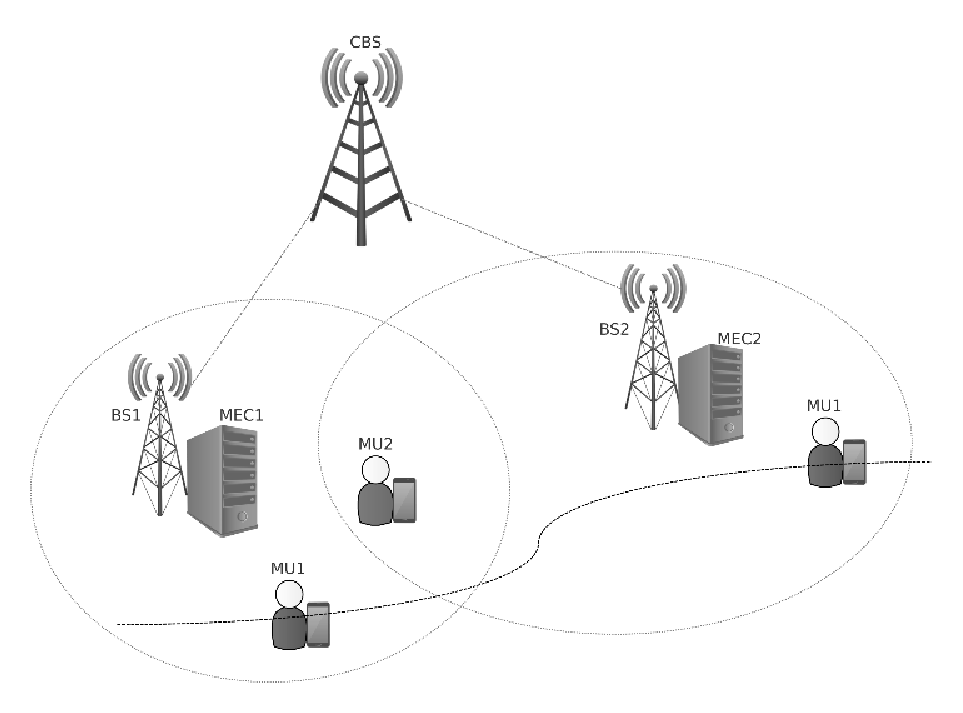
\includegraphics[width=9.5cm, height=8cm]{F1MECNetwork.eps}}
\caption{MEC Network}
\label{fig.1}
\end{figure}

  We consider $\mathbb{N}=\{1,2,\dots ,\ i,\dots ,N\}$ be the mobile users moving around the area under MEN. Each user is having a task $T_i$, denoted as a triple $(s_i,c_i,t^{max}_i)$ where $s_i$ is the size of the computational task, $c_i$ is the required computation resource (in cycles) and $t^{max}_i$ is the task deadline.  Also, there are a total of $M$ base stations each with signal range $r_j$ and the associated MEC having computation capacity $a_j$. 



\subsection{Energy Consumption and Task Delay}

\subsubsection{Task Uploading}
Mobile users first offload the task and the communication rate between user $i$ and server $j$ can be expressed as
\begin{equation} \label{c_rate}
r^u_{i,j}=B{{\mathrm{log}}_2 \left(1+\frac{p_i^td^{-\alpha }_{i,j}}{N_0B}\right) } 
\end{equation}
where $B$ indicates the channel bandwidth, $d_{i,j}$ is the distance between the user $i$ and MEC server $j$, $N_0$ is the noise power spectral density, and $\alpha $ is the channel fading parameter. The uploading time depends on the communication rate and task size and can be denoted as
\begin{equation} \label{t_upload}
t^u_{i,j}=\frac{s_i}{r^u_{i,j}} 
\end{equation}
and the uploading energy can be calculated by
\begin{equation} \label{e_upload}
e^u_{i,j}=t^u_{i,j}p^t_i
\end{equation}
where $p^t_i$ is the transmission power of mobile $i$ \\


\subsubsection{Task Transmission}
As MECs can communicate with each other by making use of CBS, the transmission rate between the server $j_1$ and $j_2$ can be expressed as 
\begin{equation} \label{t_rate}
r^{tr}_{j_1,j_2}=B{{\mathrm{log}}_2
\left(1+\frac{p_{j_1}^td^{-\alpha}_{j_1,j_2}}{N_0B}\right)}
\end{equation}
where $d_{j_1,j_2}$ is the distance between the server $j_1$ and ${j_2}_{\ }$. The transmission time and transmission energy can be formulated as
\begin{equation} \label{t_trans}
t^{tr}_{j_1,j_2}=\frac{s_i}{r^u_{j_1,j_2}}
\end{equation}
\begin{equation} \label{e_trans}
e^{tr}_{j_1,j_2}{=t}^{tr}_{j_1,j_2}p^t_{j_1}
\end{equation}
where $p^t_{j_1}$ is the transmission power of the MEC server $j_1$.\\

\subsubsection{Task Execution}
 The computation time of task $i$ in server $j$ can be denoted as
\begin{equation} \label{t_exec}
t^c_{i,j}=\frac{c_i}{a_j}
\end{equation}
and the computation energy can be calculated as 
\begin{equation} \label{e_exec}
e^c_{i,j}=t^c_{i,j}{p^{\ }_j}^c
\end{equation}
where $p^c_j$ is the computation power of MEC server $j$. 

 The download transmission delay and energy are not considered because the size of the result of the task after processing is very less and the energy consumption and delay are negligible.

\subsection{ Problem Formulation}
We assume that each user $i$ is having a task $T_i$ which can be offloaded. As the user is moving, the MECs to which user $i$ can offload the task varies with time and we denote $S^t_i$ as the set of available MECs at time $t$ and let $mt_i$ be the total time user $i$ is moving. We aim to find a MEC server $j$ from the set of available servers in user $i's$ trajectory  ${i.e.,S_i=\{\bigcup^{mt_i}_{t=0}{S^t_i\}},}$satisfying task $i's$ deadline to minimize the total energy consumption. The task offloading problem can then be modelled as
 
\[P1: \begin{array}{c}
 \begin{array}{c}
{\mathrm{min} \sum_{i\in N}{\sum_{j\in S_i}x_{i,j}E_{i,j}}} \\ \\
 \begin{array}{cc}
s.t. & C1:{\ t}_{i,j}\le t^{max}_i\ ,\forall i\in N \\ \\
\  & C2:\sum_{j\in S_i}{x_{i,j}}=1\ ,\forall i\in N \\ \\
\  & C3:x_{i,j}\in \{0,1\}\  \end{array} \\ \\
 \end{array}
 \end{array}
\] 

 It's very clear from the conditions $C2,\ C3$ that the task $T_i$ should be computed only once at some server $j\in S_i$ and can't be divided. 

  The energy $E_{i,j}$ and time $t_{i,j}$ in the above formulation can be expressed as
\begin{equation} \label{t_total}
E_{i,j}=e^u_{i,j_1}+\sum^{t_2}_{t=t_1}e^{tr}_{{j\in S_i^t},{j\in S_i^{t+1}}} +e^c_{i,j} 
\end{equation}

\begin{equation} \label{e_total}
t_{i,j}=t^u_{i,j_1}+\sum^{t_2}_{t=t_1}t^{tr}_{{j\in S_i^t},{j\in S_i^{t+1}}} +t^c_{i,j} 
\end{equation}

\[ \begin{array}{cc}
\  &  \begin{array}{cc}
where & j_1\in S^0_i \\ 
\  & 0\le t_1<t_2<mt_i \\ 
\  & j \in S^{t_2+1}_i \end{array}
 \end{array}
\] 

\eqref{t_total} and \eqref{e_total} indicates that total energy and total time includes energy and time spent in uploading, transmission, and computation of a task.



\begin{table}[htbp]
\caption{Symbols Description}
\begin{center}
\begin{tabular}{|p{0.6in}|p{2.5in}|}
\hline
\textbf{Symbol}&\textbf{Description}\\
\hline
$s_i$ & size of the computational task $T_i$  \\
\hline
$c_i$ & computation resource (in cycles) needed for task $T_i$ \\
\hline
$t_i^{max}$ & deadline for task $T_i$ \\
\hline
$r_j$ & signal range of MEC server $j$ \\
\hline
$a_j$ & computation capacity of MEC server $j$ \\
\hline
$r^u_{i,j}$ & communication rate between user $i$ and server $j$ \\
\hline
$r^{tr}_{j_1,j_2}$ & transmission rate between servers $j_1$and $j_2$ \\
\hline
$B$ & channel bandwidth \\
\hline
$N_0$ & noise power spectral density \\
\hline
$\alpha$ & channel fading parameter \\
\hline
$t^u_{i,j}, e^u_{i,j}$ & delay and energy consumption for task uploading from user $i$ to server $j$ \\
\hline
$t^{tr}_{j_1,j_2}, e^{tr}_{j_1,j_2}$ & delay and energy consumption for task transmission between servers $j_1$and $j_2$ \\
\hline
$t^c_{i,j}, e^c_{i,j}$ & delay and energy consumption for execution of a task from user $i$ in server $j$  \\
\hline
$d_{i,j}$ & distance between user $i$ and MEC server $j$ \\
\hline
$p_i^t$ & transmission power of user mobile $i$ \\
\hline
$p_j^t$ & transmission power of server $j$ \\
\hline
$p_j^c$ & computation power of server $j$ \\
\hline
\end{tabular}
\label{table.1}
\end{center}
\end{table}


\section{ Proposed Algorithm}

 The above problem $P1$ is a constraint-satisfaction problem and it is NP-complete. We propose a heuristic to solve the problem and it is as follows: 

 Each user $i$ offloads task $T_i$ with the required information: size of the computational task, required computation resource (in cycles) and the task deadline. The CBS then assigns each task to a MEC server satisfying task deadline and least energy consumption. The delay constrained energy minimal task offloading algorithm shortly referred to as DCEMTO algorithm is shown in Algorithm 1. 

 For each user $i\in N$, at each time step $t\in {[0,mt_i]}$, available MEC servers $S^t_i$ is found out. Among the servers in $S^t_i$, our goal is to find out two servers, one for execution to which task can be assigned and one for transmission from which task can be offloaded to a server $({\in S}^{t+1}_i)$  situated in the next time step locality. As the task assignment has to satisfy delay constraint, the time needed for uploading, transmission, and execution is also calculated and checked for delay constraint in each timestep.

 For each available server $(\in S^t_i)$, the energy consumed due to transmission (up to timestep $t-1$), and execution is calculated. This process is repeated for all time steps and the server with the least energy is assigned to the task $T_i$ for execution. 

 The energy consumed due to transmission at timestep $t$ can be found out by adding transmission energy up to timestep $t-1$ and energy needed to offload task from server's location to user's locality in next time step $t+1$. 

 In the end, the algorithm outputs $x_i \forall i \in N$, the energy-optimal server satisfying delay constraint of task $T_i$. 
 
 \begin{algorithm}
 \caption{DCEMTO Algorithm}
 \begin{algorithmic}[1]
 \renewcommand{\algorithmicrequire}{\textbf{Input: mobile users $N$, base stations $M$}}
 \renewcommand{\algorithmicensure}{\textbf{Output: $x_i ,\forall i \in M$}}
 \REQUIRE 
 \ENSURE  

  \FOR{\textbf{each } user $i \in N$}
  \FOR{\textbf{each } timestep  $t \in {[0,mt_i]}$}
  \STATE $S_i^t \mathrm{\leftarrow }$ get available MEC servers at timestep $t$
  \FOR{\textbf{each } server  $j \in S_i^t$}
  \IF {$t == 0$}
  \STATE $t^c_j=t^u_{i,j}+t^c_{i,j}$
  \IF {$t^c_j\le td_i$}
  \STATE $e^c_j=e^u_{i,j}+e^c_{i,j}$
  \ELSE
  \STATE $e^c_j \mathrm{\leftarrow } \mathrm{\infty }$
  \ENDIF
  \ELSE
  \STATE $t^c_j=t^{tr}_{j_{0\dots t-1}}+t^{tr}_{j_{t-1},j}+t^c_{i,j}$
  \IF {$t^c_j\le td_i$}
  \STATE $e^c_j=t^{tr}_{j_{0\dots t-1}}+e^{tr}_{j_{t-1},j}+e^c_{i,j}$
  \ELSE
  \STATE $e^c_j \mathrm{\leftarrow } \mathrm{\infty }$
  \ENDIF
  \ENDIF
  \ENDFOR
  \STATE $j^t_*=argmin_j(e^c_j)$
  \STATE let $k$ be the user $i's$ trajectory at $t+1$
  \FOR{\textbf{each } server  $j \in S_i^t$}
  \STATE $e^t_{j,k}=\frac{p_jd_{j,k}}{r_{j,k}}$
  \ENDFOR
  
  \STATE $j_t=argmin_j(e^t_{j,k})$
  \STATE $ e^{tr}_{j_{0..t}}=e^{tr}_{j_{0..t-1}}+e^{tr}_{j_{t-1},j_t}$
  \STATE $t^{tr}_{j_{0..t}}=t^{tr}_{j_{0..t-1}}+t^{tr}_{j_{t-1},j_t}$
 
  \ENDFOR
  \STATE $x_i=argmin_{j_*}(e^c_{j^t_*})$
  \ENDFOR
 \RETURN $x_i ,\forall i \in M$ 
 \end{algorithmic} 
 \end{algorithm}
 
 
\begin{table}
\caption{Simulation Parameters}
\begin{center}
\begin{tabular}{|c|c|}
\hline
\textbf{Parameters}&\textbf{Value/Range}\\
\hline
Coverage radius of BS & 70 to 100 meters  \\
\hline
MEC’s CPU capacity & [7, 20] GHz \\
\hline
MEC’s computation power  & [3,5] watt \\
\hline
MEC’s transmission power & [0.1,1] watt \\
\hline
Channel bandwidth & 1MHz \\
\hline
User’s mobility speed & 1$\mathrm{\sim}$3 MPH \\
\hline
Task CPU requirement & [1,10] GHz \\
\hline
Input data size & [1,3] MB \\
\hline
Task deadline constraint & [0.1,1] sec \\
\hline
\end{tabular}
\label{table.2}
\end{center}
\end{table}
 
\section{Evaluation}

\begin{figure}
\centerline{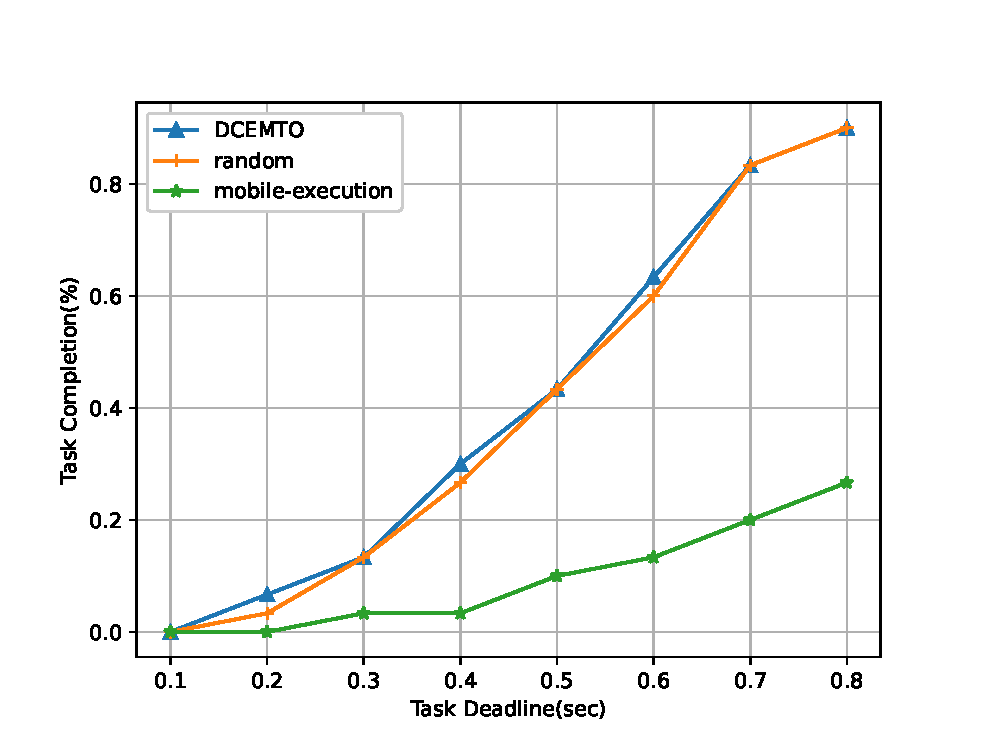
\includegraphics[width=9.5cm, height=7cm]{F2TaskCompletionvsDeadline.eps}}
\caption{Task Completion \% vs Task Deadline}
\label{fig.2}
\end{figure}

\begin{figure}
\centerline{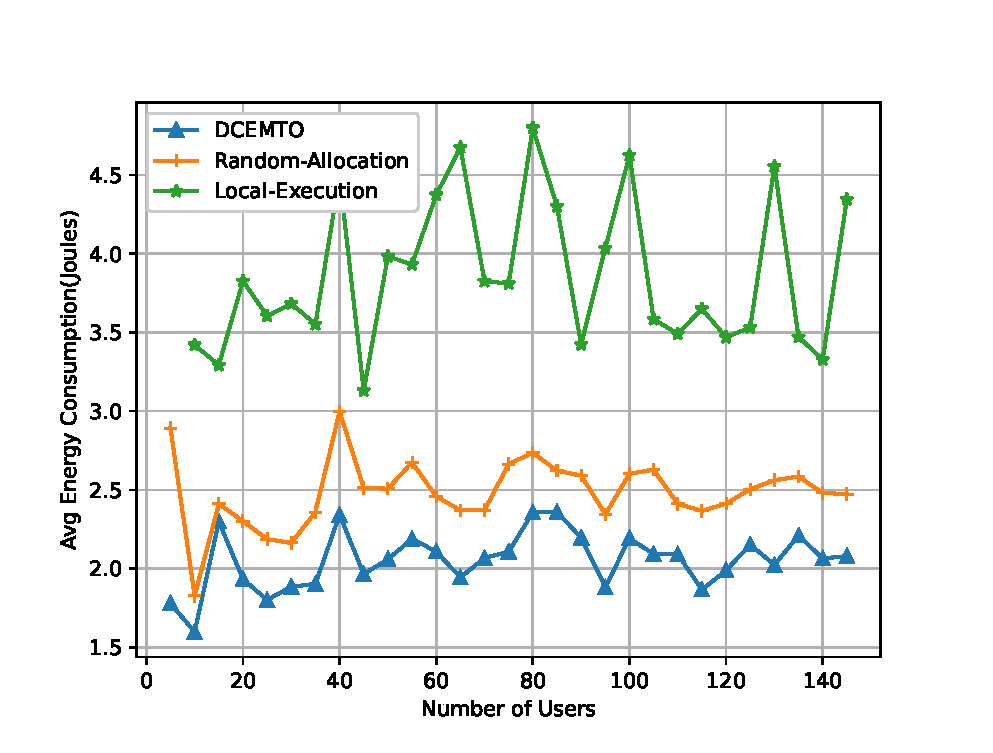
\includegraphics[width=9.5cm, height=7cm]{F3AvgECvsNoUsers.eps}}
\caption{Avg Energy Consumption vs Number of Users}
\label{fig.3}
\end{figure}

\begin{figure}
\centerline{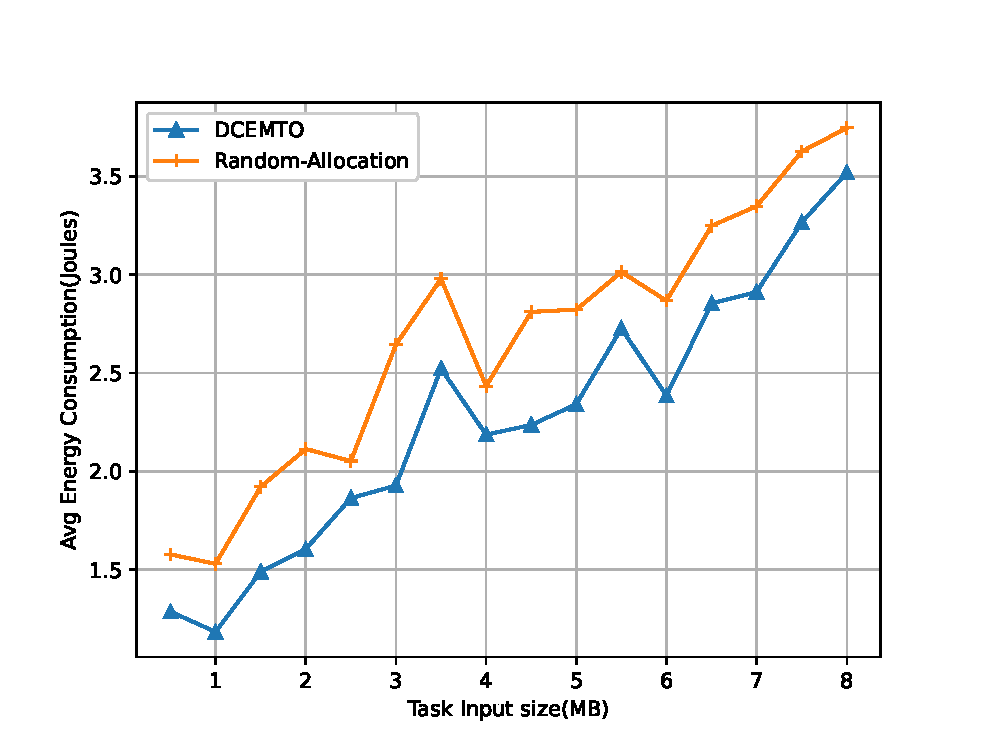
\includegraphics[width=9.5cm, height=7cm]{F4TaskSizevsAvgEC.eps}}
\caption{Task Input Size vs Energy Consumption}
\label{fig.4}
\end{figure}

In this section, we evaluated the performance of our proposed algorithm to achieve energy minimal task offloading with users’ mobility and delay constraints into consideration. we used data of base stations within the Melbourne central business district area in Australia, which has a total area of 6.2 $km^2$ provided by the Australian Communications and Media Authority \cite{b6}. There are a total of 126 base stations situated inside the Melbourne CBD area.
	We follow the Random waypoint mobility model for the users moving in the area covered by the base stations provided in the dataset. The random waypoint model is a random model for the movement of mobile users, and how their location, velocity and acceleration change over time. 
	Without loss of generality, we refer to the parameter settings in the existing works \cite{b2}, \cite{b7}. The coverage radius of BS is randomly taken varying from 70 to 100 meters and the associated MEC’s CPU capacity is in [7, 20] GHz, computation power is in [3,5] watts and transmission power ranges from 0.1 to 1 watt. The bandwidth of the communication channel is set up as 1MHz. Users are moving with the speed of 1~3 MPH and generate tasks with input data size varies from 1 MB to 3 MB having CPU requirement is in [1,10] GHz and deadline constraint within [0.1,1] seconds. Users’ mobiles are having CPU capacity ranges from 1 to 10 GHz, transmission power is randomly taken from [7,15] watts and computation power from [7,10] watts. We consider mobile-execution and random-allocation as our baseline algorithms:
	


\begin{itemize}
\item Local-Execution: Feasible Tasks satisfying delay constraint are executed within the mobiles without offloading. 
\item Random-Allocation: Each user’s task is assigned to a server randomly chosen from the servers present along the user’s trajectory.
\end{itemize}


 
Fig. 2 depicts the higher Task completion percentage compared to the other 2 approaches by varying Task deadline constraint. DCEMTO’s task completion is 9.16\% higher than Random-Allocation and 27.08\% higher than Local-Execution on average. Also, Task completion percentage increases by increasing Deadline constraint.

	Fig. 3 indicates the variation of average energy consumption with a change in the number of users. DCEMTO outperforms other approaches. Average energy consumption in DCEMTO is 10.5\% energy efficient than Random-Allocation and 46.5\% efficient than Local-Execution. 


Fig. 4 shows how energy consumption varies with varying task input size. It’s clear that higher the task input size, energy consumption increases. It is due to higher transmission energy needed in task offloading. Energy consumption in DCEMTO is 9.55\% efficient than Random-Allocation approach.


\section{Conclusion}
In this paper, we explored the problem of Energy-minimal task offloading in the Mobile Edge Computing environment by considering the mobility of users and task deadline constraint. We mathematically formulated the problem and proposed a heuristic algorithm DCEMTO, where user mobility, task deadline and base station information are utilized to optimize the overall energy consumption for task execution. We evaluated our algorithm on Melbourne CBD base stations dataset by comparing with baseline approaches like Random-Allocation and Local-Execution. The results convey that our DCEMTO algorithm outperforms other approaches in metrics like Task Acceptance rate, Average Energy consumption and overall Energy Consumption.

\begin{thebibliography}{00}
\bibitem{b1} J. Wang, W. Wu, Z. Liao, A. K. Sangaiah and R. Simon Sherratt, "An Energy-Efficient Off-Loading Scheme for Low Latency in Collaborative Edge Computing," in IEEE Access, vol. 7, pp. 149182-149190, 2019.
\bibitem{b2} Y. Kai, J. Wang and H. Zhu, "Energy Minimization for D2D-Assisted Mobile Edge Computing Networks," ICC 2019 - 2019 IEEE International Conference on Communications (ICC), Shanghai, China, 2019, pp. 1-6.
\bibitem{b3} C. Wu, Q. Peng, Y. Xia and J. Lee, "Mobility-Aware Tasks Offloading in Mobile Edge Computing Environment," 2019 Seventh International Symposium on Computing and Networking (CANDAR), Nagasaki, Japan, 2019, pp. 204-210.
\bibitem{b4} Z. Liu, X. Wang, D. Wang, Y. Lan and J. Hou, "Mobility-aware Task Offloading and Migration Schemes in SCNs with Mobile Edge Computing," 2019 IEEE Wireless Communications and Networking Conference (WCNC), Marrakesh, Morocco, 2019, pp. 1-6.
\bibitem{b5} Zi Wang, Zhiwei Zhao, Geyong Min, Xinyuan Huang, Qiang Ni, Rong Wang, User mobility aware task assignment for Mobile Edge Computing, Future Generation Computer Systems, Volume 85, 2018, Pages 1-8, ISSN 0167-739X.
\bibitem{b6} P. Lai, Q. He, M. Abdelrazek, F. Chen, J. Hosking, J. Grundy, and Y. Yang, “Optimal edge user allocation in edge computing with variable sized vector bin packing,” in International Conference on Service-Oriented Computing. Springer, 2018, pp. 230–245.
\bibitem{b7} Q. Peng et al., "Mobility-Aware and Migration-Enabled Online Edge User Allocation in Mobile Edge Computing," 2019 IEEE International Conference on Web Services (ICWS), Milan, Italy, 2019, pp. 91-98.
\end{thebibliography}


\end{document}
